\chapter{Elder Heliosystem Activation Functions}

\begin{tcolorbox}[colback=DarkSkyBlue!5!white,colframe=DarkSkyBlue!75!black,title=Chapter Summary]
This chapter presents a mathematical framework for specialized activation functions within the Elder Heliosystem, examining the requirements of complex-valued computations and phase-sensitive operations. We describe formulations of activation functions designed for the Elder paradigm, analyzing their properties, implementation considerations, and theoretical aspects. The chapter examines tensor-based formulations of complex-domain activation functions that relate to phase coherence while modulating magnitude, presents gradient formulations for backpropagation, and analyzes their computational characteristics. The mathematical analysis considers how these specialized activation functions relate to several capabilities: maintaining phase relationships that encode temporal and hierarchical information, affecting orbital selection of subnetworks based on phase alignment, relating to cross-modal integration across domains, and modeling uncertainty through phase diffusion. These activation functions function as components of the Elder computational architecture, providing non-linearities while maintaining the phase relationships that are part of the system's operation.
\end{tcolorbox}

\section{Introduction to Complex Activation Functions}

Standard neural networks employ activation functions that operate on real-valued inputs, producing real-valued outputs to introduce non-linearities. However, the Elder Heliosystem operates in a fundamentally different computational paradigm, requiring specialized activation functions that leverage complex-valued representations and phase relationships.

These complex-domain activation functions serve multiple crucial purposes in the Elder Heliosystem:

\begin{enumerate}
    \item \textbf{Phase Coherence Preservation}: Maintaining meaningful phase relationships that encode temporal and hierarchical information
    \item \textbf{Magnitude Modulation}: Controlling signal strength while preserving directional information
    \item \textbf{Orbital Selection}: Activating specific subnetworks based on phase relationships
    \item \textbf{Cross-Modal Integration}: Enabling information transfer across different domains and modalities
    \item \textbf{Uncertainty Representation}: Encoding uncertainty through phase diffusion
\end{enumerate}

This chapter presents the mathematical formulations, properties, and specific applications of activation functions uniquely designed for the Elder Heliosystem architecture.

\section{Complex-Valued Activation Functions}

\subsection{Helical Activation Function (HAF)}

The Helical Activation Function forms the cornerstone of the Elder Heliosystem's non-linear processing capabilities, enabling phase-coherent learning while providing controlled non-linearities.

\begin{definition}[Helical Activation Function]
For a complex input $z \in \mathbb{C}$, the Helical Activation Function is defined as:
\begin{equation}
\text{HAF}(z) = z \cdot e^{i\phi(|z|)}
\end{equation}
where $\phi(|z|) = \alpha \cdot \tanh(\beta|z|)$ with hyperparameters $\alpha$ controlling the maximum phase rotation and $\beta$ controlling the sensitivity to magnitude.
\end{definition}

\begin{figure}[h]
\centering
\begin{tikzpicture}[scale=2.5]
    % Axes
    \draw[->] (-1.2,0) -- (1.2,0) node[right] {$\text{Re}(z)$};
    \draw[->] (0,-1.2) -- (0,1.2) node[above] {$\text{Im}(z)$};
    
    % Unit circle
    \draw[dashed] (0,0) circle (1);
    
    % Input vectors
    \draw[->,blue,thick] (0,0) -- (0.7,0.4) node[midway,above] {$z$};
    
    % HAF output
    \draw[->,red,thick] (0,0) -- (0.5,0.6) node[midway,right] {$\text{HAF}(z)$};
    
    % Angle indication
    \draw[->] (0.3,0) arc (0:40:0.3) node[midway,right] {$\phi(|z|)$};
\end{tikzpicture}
\caption{Visualization of the Helical Activation Function showing how it preserves magnitude while rotating phase}
\end{figure}

The HAF preserves the magnitude of the input while applying a magnitude-dependent phase rotation, creating a helical transformation pattern in the complex plane. This enables rich non-linear transformations while maintaining important phase relationships.

\begin{theorem}[HAF Properties]
The Helical Activation Function exhibits the following properties:
\begin{enumerate}
    \item \textbf{Magnitude Preservation}: $|\text{HAF}(z)| = |z|$
    \item \textbf{Phase Modulation}: $\arg(\text{HAF}(z)) = \arg(z) + \phi(|z|)$
    \item \textbf{Differentiability}: HAF is differentiable everywhere except at $z=0$
    \item \textbf{Bounded Phase Shift}: $\lim_{|z| \to \infty} \phi(|z|) = \alpha$
\end{enumerate}
\end{theorem}

HAF serves as the primary activation function in the highest levels of the Elder component, where preserving phase coherence while introducing non-linearities is critical for stable learning dynamics.

\subsection{Phase-Preserving ReLU (PP-ReLU)}

The Phase-Preserving ReLU extends the popular ReLU activation function to complex-valued domains while preserving phase information critical to the Elder Heliosystem.

\begin{definition}[Phase-Preserving ReLU]
For a complex input $z \in \mathbb{C}$, the Phase-Preserving ReLU is defined as:
\begin{equation}
\text{PP-ReLU}(z) = \max(|z|, 0) \cdot e^{i\arg(z)}
\end{equation}
\end{definition}

Unlike standard ReLU which would discard all phase information for negative real inputs, PP-ReLU preserves the directional information encoded in the phase while applying thresholding to the magnitude.

\begin{observation}
PP-ReLU reduces to standard ReLU when restricted to the real domain:
\begin{equation}
\text{PP-ReLU}(x) = \max(x, 0) \quad \text{for} \quad x \in \mathbb{R}
\end{equation}
\end{observation}

This activation function is commonly employed in Mentor entities where magnitude thresholding provides beneficial sparsity while maintaining critical phase relationships with the Elder and Erudite entities.

\subsection{Orbital Activation Function (OAF)}

The Orbital Activation Function enables phase-conditional computation by selectively activating signals based on their phase alignment with the Elder phase.

\begin{definition}[Orbital Activation Function]
For a complex input $z \in \mathbb{C}$ and Elder phase $\phi_E$, the Orbital Activation Function is defined as:
\begin{equation}
\text{OAF}(z, \phi_E) = z \cdot \frac{1 + \cos(\arg(z) - \phi_E)}{2}
\end{equation}
\end{definition}

OAF attenuates signals whose phases are far from the current Elder phase while amplifying those closely aligned. This enables the system to focus computational resources on phase-relevant information processing.

\begin{figure}[h]
\centering
\begin{tikzpicture}[scale=2.5]
    % Axes
    \draw[->] (-1.2,0) -- (1.2,0) node[right] {$\text{Re}(z)$};
    \draw[->] (0,-1.2) -- (0,1.2) node[above] {$\text{Im}(z)$};
    
    % Unit circle
    \draw[dashed] (0,0) circle (1);
    
    % Elder phase reference
    \draw[->,green!60!black,thick] (0,0) -- (0.866,0.5) node[midway,above] {$\phi_E$};
    
    % Input vectors at different phase distances
    \draw[->,blue,thick] (0,0) -- (0.866,0.5) node[right] {$z_1$};
    \draw[->,blue,thick] (0,0) -- (0.5,-0.866) node[right] {$z_2$};
    
    % OAF outputs
    \draw[->,red,thick] (0,0) -- (0.866,0.5) node[above right] {\tiny $\text{OAF}(z_1)$};
    \draw[->,red,thick] (0,0) -- (0.25,-0.433) node[below right] {\tiny $\text{OAF}(z_2)$};
\end{tikzpicture}
\caption{Orbital Activation Function selectively attenuates signals based on phase distance from Elder phase $\phi_E$}
\end{figure}

The OAF is a core function for implementing phase-conditional computation in Erudites, enabling the system to achieve extreme sparsity by selectively activating only phase-relevant pathways.

\section{Phase-Based Activation Functions}

\subsection{Resonant Wave Activation (RWA)}

The Resonant Wave Activation function combines standard sigmoid activation with phase-dependent oscillatory components to enable rich cross-domain information transfer.

\begin{definition}[Resonant Wave Activation]
For a real input $x \in \mathbb{R}$ and phase parameter $\phi$, the Resonant Wave Activation is defined as:
\begin{equation}
\text{RWA}(x, \phi) = \sigma(x) \cdot (1 + \alpha \cdot \sin(\omega x + \phi))
\end{equation}
where $\sigma$ is the sigmoid function, and hyperparameters $\alpha \in [0,1]$ and $\omega > 0$ control the oscillation amplitude and frequency, respectively.
\end{definition}

RWA introduces phase-modulated oscillatory behavior to the standard sigmoid, creating resonant patterns that facilitate information transfer across different Mentor domains within the Elder Heliosystem.

\begin{figure}[h]
\centering
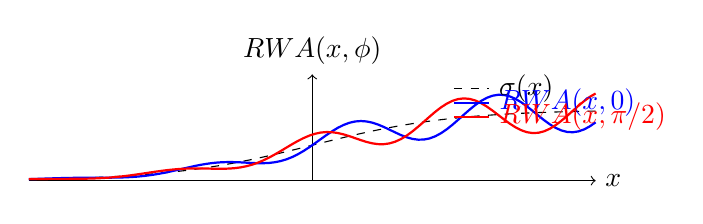
\begin{tikzpicture}[scale=0.9]
    % Axes
    \draw[->] (-4,0) -- (4,0) node[right] {$x$};
    \draw[->] (0,0) -- (0,1.5) node[above] {$\text{RWA}(x,\phi)$};
    
    % Draw sigmoid
    \draw[dashed] plot[domain=-4:4,samples=100] (\x,{1/(1+exp(-\x))});
    
    % Draw RWA with different phases
    \draw[blue,thick] plot[domain=-4:4,samples=100] (\x,{1/(1+exp(-\x))*(1 + 0.3*sin(3*\x*180/3.14159))});
    \draw[red,thick] plot[domain=-4:4,samples=100] (\x,{1/(1+exp(-\x))*(1 + 0.3*sin(3*\x*180/3.14159 + 90))});
    
    % Legend
    \draw[dashed] (2,1.3) -- (2.5,1.3) node[right] {$\sigma(x)$};
    \draw[blue,thick] (2,1.1) -- (2.5,1.1) node[right] {$\text{RWA}(x,0)$};
    \draw[red,thick] (2,0.9) -- (2.5,0.9) node[right] {$\text{RWA}(x,\pi/2)$};
\end{tikzpicture}
\caption{Resonant Wave Activation function with different phase values compared to standard sigmoid}
\end{figure}

\begin{proposition}[RWA Properties]
The Resonant Wave Activation function exhibits the following properties:
\begin{enumerate}
    \item \textbf{Bounded Output}: $\text{RWA}(x, \phi) \in [0, 1+\alpha]$ for positive $\alpha$
    \item \textbf{Phase Sensitivity}: $\frac{\partial\text{RWA}}{\partial\phi} = -\alpha \cdot \sigma(x) \cdot \cos(\omega x + \phi)$
    \item \textbf{Oscillatory Gradient}: Gradient exhibits periodic variations enhancing exploration during learning
\end{enumerate}
\end{proposition}

RWA is primarily used for cross-domain information transfer between different Mentor domains, where the phase parameters encode domain-specific characteristics.

\subsection{Phase-Selective Gate (PSG)}

The Phase-Selective Gate provides a mechanism for filtering Erudite outputs based on their phase distance from a reference phase.

\begin{definition}[Phase-Selective Gate]
For an input $x \in \mathbb{R}$, current phase $\phi$, reference phase $\phi_{\text{ref}}$, and sensitivity parameter $\gamma > 0$:
\begin{equation}
\text{PSG}(x, \phi, \phi_{\text{ref}}) = x \cdot \text{softmax}(-\gamma \cdot d_{\text{circ}}(\phi, \phi_{\text{ref}}))
\end{equation}
where $d_{\text{circ}}(\phi_1, \phi_2) = \min(|\phi_1 - \phi_2|, 2\pi - |\phi_1 - \phi_2|)$ is the circular distance between phases.
\end{definition}

PSG incorporates a soft gating mechanism that attenuates signals based on phase distance, enabling selective propagation of information during different phases of processing.

\begin{observation}
As $\gamma \to \infty$, PSG approaches a hard phase gate that completely blocks signals when phases differ beyond a threshold.
\end{observation}

This activation is critical for implementing the phase-selective processing paradigm fundamental to the Elder Heliosystem's computational efficiency.

\subsection{Harmonic Basis Activation (HBA)}

The Harmonic Basis Activation decomposes the activation into multiple harmonic components, enabling rich feature extraction across different frequency domains.

\begin{definition}[Harmonic Basis Activation]
For input $x \in \mathbb{R}$ and a set of phase parameters $\{\phi_k\}_{k=1}^n$:
\begin{equation}
\text{HBA}(x, \{\phi_k\}_{k=1}^n) = \sum_{k=1}^n w_k \cdot \sigma(x) \cdot \sin(k\phi_k)
\end{equation}
where $w_k$ are learnable weights and $\sigma$ is the sigmoid function.
\end{definition}

HBA performs a harmonic decomposition of the activation signal, analogous to a Fourier series with learnable coefficients. This enables feature extraction across multiple frequency bands, critical for processing complex temporal patterns.

\begin{theorem}[Representation Power]
Any continuous function $f: [0,1] \times [0,2\pi] \to \mathbb{R}$ can be approximated to arbitrary precision using HBA with sufficient harmonic components.
\end{theorem}

HBA is primarily employed in Erudite-level processing for feature decomposition in temporal and spectral domains.

\section{Specialized Hierarchical Activations}

\subsection{Elder-Mentor Coupling Function (EMCF)}

The Elder-Mentor Coupling Function enables guided learning through phase synchronization between Elder and Mentor entities.

\begin{definition}[Elder-Mentor Coupling Function]
For Elder state $z_E \in \mathbb{C}$, Mentor state $z_M \in \mathbb{C}$, and coupling strength $\alpha > 0$:
\begin{equation}
\text{EMCF}(z_E, z_M) = z_M + \alpha \cdot z_E \cdot \sin(\arg(z_E) - \arg(z_M))
\end{equation}
\end{definition}

EMCF applies a corrective force that pulls the Mentor phase toward alignment with the Elder phase, with strength proportional to the phase difference. This enables hierarchical guidance while maintaining Mentor autonomy.

\begin{figure}[h]
\centering
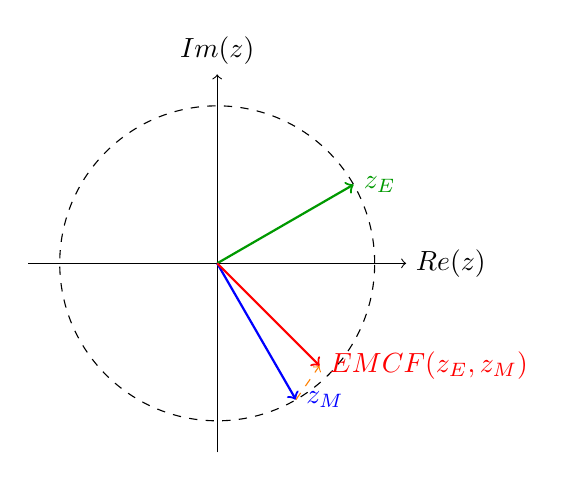
\begin{tikzpicture}[scale=2]
    % Axes
    \draw[->] (-1.2,0) -- (1.2,0) node[right] {$\text{Re}(z)$};
    \draw[->] (0,-1.2) -- (0,1.2) node[above] {$\text{Im}(z)$};
    
    % Unit circle
    \draw[dashed] (0,0) circle (1);
    
    % Input vectors
    \draw[->,green!60!black,thick] (0,0) -- (0.866,0.5) node[right] {$z_E$};
    \draw[->,blue,thick] (0,0) -- (0.5,-0.866) node[right] {$z_M$};
    
    % EMCF output
    \draw[->,red,thick] (0,0) -- (0.65,-0.65) node[right] {$\text{EMCF}(z_E,z_M)$};
    
    % Force vector
    \draw[->,orange,dashed] (0.5,-0.866) -- (0.65,-0.65);
\end{tikzpicture}
\caption{Elder-Mentor Coupling Function showing how Elder state influences Mentor state through phase-based coupling}
\end{figure}

\begin{proposition}[Phase Convergence]
Under repeated application of EMCF with constant $z_E$, the phase of $z_M$ converges to the phase of $z_E$ within a bounded number of steps for any $\alpha > 0$.
\end{proposition}

EMCF serves as the primary mechanism for Elder influence on Mentors, enabling knowledge transfer while maintaining the magnitude characteristics of the Mentor state.

\subsection{Mentor-Erudite Transfer Function (METF)}

The Mentor-Erudite Transfer Function facilitates knowledge transfer from Mentors to Erudites through phase-based amplification.

\begin{definition}[Mentor-Erudite Transfer Function]
For Mentor state $z_M \in \mathbb{C}$, Erudite state $z_E \in \mathbb{C}$, and transfer strength $\beta > 0$:
\begin{equation}
\text{METF}(z_M, z_E) = z_E \cdot (1 + \beta \cdot \cos(\arg(z_M) - \arg(z_E)))
\end{equation}
\end{definition}

METF amplifies Erudite activations that align with the Mentor phase, creating a phase-selective learning channel from Mentor to Erudite.

\begin{proposition}[METF Properties]
The Mentor-Erudite Transfer Function has the following properties:
\begin{enumerate}
    \item \textbf{Phase Alignment Amplification}: Maximum gain occurs when $\arg(z_M) = \arg(z_E)$
    \item \textbf{Phase Opposition Suppression}: Minimum gain occurs when $\arg(z_M) = \arg(z_E) \pm \pi$
    \item \textbf{Magnitude Modulation Range}: Output magnitude ranges from $(1-\beta)|z_E|$ to $(1+\beta)|z_E|$
\end{enumerate}
\end{proposition}

METF is the core mechanism for knowledge transfer from Mentors to Erudites, enabling selective enhancement of aligned activations while suppressing misaligned ones.

\subsection{Multi-Orbital Gating Function (MOGF)}

The Multi-Orbital Gating Function enables integration of knowledge from multiple orbiting entities based on their phase relevance.

\begin{definition}[Multi-Orbital Gating Function]
For a set of input states $\{z_i\}_{i=1}^n$, phases $\{\phi_i\}_{i=1}^n$, current system phase $\phi_{\text{curr}}$, and sensitivity parameter $\lambda > 0$:
\begin{equation}
\text{MOGF}(\{z_i\}_{i=1}^n, \{\phi_i\}_{i=1}^n) = \sum_{i=1}^n z_i \cdot \text{softmax}_i(-\lambda \cdot d_{\text{circ}}(\phi_i, \phi_{\text{curr}}))
\end{equation}
where $\text{softmax}_i$ denotes the softmax function applied across the index $i$.
\end{definition}

MOGF creates a soft attention mechanism over multiple entities based on their phase proximity to the current system phase, enabling dynamic routing of information.

\begin{theorem}[Phase-Based Routing]
MOGF implements a differentiable router that selectively combines information from multiple sources based on phase proximity, with the following properties:
\begin{enumerate}
    \item \textbf{Phase-Selective Attention}: Sources with phases closer to $\phi_{\text{curr}}$ receive higher attention weights
    \item \textbf{Normalized Contribution}: Attention weights sum to 1, ensuring stable integration
    \item \textbf{Smooth Phase Transition}: As $\phi_{\text{curr}}$ evolves, attention smoothly transitions between sources
\end{enumerate}
\end{theorem}

MOGF is employed for integration of knowledge from multiple orbiting entities, especially when combining outputs from multiple Mentors to influence the Elder's state.




\section{Relationship to the Elder Heliosystem's Gravitational Model}

The activation functions presented in this chapter implement critical aspects of the Elder Heliosystem's fundamental gravitational model. While the gravitational stabilization mechanism is fully explained in Chapter 6 (The Elder Heliosystem: A Unified Closed System), these activation functions provide the mathematical operations necessary to implement this mechanism in practice.

The Elder-Mentor Coupling Function (EMCF) and Mentor-Erudite Transfer Membranes (METM) are particularly important as they directly implement the gravitational influence that maintains stable orbital relationships between hierarchical entities. These transfer membranes apply corrective forces that prevent orbital decay by synchronizing phases when they begin to drift, enabling the perpetuation of stable revolutionary orbits essential to the system's learning ability.

Transfer membranes represent a more accurate conceptual framework than "transfer orbits" because they:
\begin{itemize}
    \item Act as semi-permeable boundaries that selectively allow knowledge to pass between hierarchical levels
    \item Maintain phase coherence during knowledge transitions
    \item Provide controlled resistance that prevents catastrophic knowledge collapse
    \item Enable bidirectional information flow while preserving hierarchical structure
\end{itemize}

\section{Future Directions}

Research into Elder Heliosystem activation functions continues to explore several promising directions:

\begin{enumerate}
    \item \textbf{Higher-dimensional Complex Functions}: Extending to quaternion and octonion spaces for richer representations
    \item \textbf{Phase-Adaptive Activations}: Self-modifying functions that adapt their parameters based on system state
    \item \textbf{Geometric Activation Functions}: Incorporating non-Euclidean geometries like hyperbolic and spherical spaces
    \item \textbf{Spiking Neural Network Inspiration}: Drawing from neuromorphic computing to implement energy-efficient phase-coded activations
    \item \textbf{Quantum Circuit Emulation}: Using complex activations to emulate aspects of quantum circuits for specialized tasks
\end{enumerate}

These directions promise to further enhance the Elder Heliosystem's capabilities across diverse application domains, from multimodal integration to uncertainty quantification and causal reasoning.